
% Default to the notebook output style

    


% Inherit from the specified cell style.




    
\documentclass[11pt]{article}

    
    
    \usepackage[T1]{fontenc}
    % Nicer default font (+ math font) than Computer Modern for most use cases
    \usepackage{mathpazo}

    % Basic figure setup, for now with no caption control since it's done
    % automatically by Pandoc (which extracts ![](path) syntax from Markdown).
    \usepackage{graphicx}
    % We will generate all images so they have a width \maxwidth. This means
    % that they will get their normal width if they fit onto the page, but
    % are scaled down if they would overflow the margins.
    \makeatletter
    \def\maxwidth{\ifdim\Gin@nat@width>\linewidth\linewidth
    \else\Gin@nat@width\fi}
    \makeatother
    \let\Oldincludegraphics\includegraphics
    % Set max figure width to be 80% of text width, for now hardcoded.
    \renewcommand{\includegraphics}[1]{\Oldincludegraphics[width=.8\maxwidth]{#1}}
    % Ensure that by default, figures have no caption (until we provide a
    % proper Figure object with a Caption API and a way to capture that
    % in the conversion process - todo).
    \usepackage{caption}
    \DeclareCaptionLabelFormat{nolabel}{}
    \captionsetup{labelformat=nolabel}

    \usepackage{adjustbox} % Used to constrain images to a maximum size 
    \usepackage{xcolor} % Allow colors to be defined
    \usepackage{enumerate} % Needed for markdown enumerations to work
    \usepackage{geometry} % Used to adjust the document margins
    \usepackage{amsmath} % Equations
    \usepackage{amssymb} % Equations
    \usepackage{textcomp} % defines textquotesingle
    % Hack from http://tex.stackexchange.com/a/47451/13684:
    \AtBeginDocument{%
        \def\PYZsq{\textquotesingle}% Upright quotes in Pygmentized code
    }
    \usepackage{upquote} % Upright quotes for verbatim code
    \usepackage{eurosym} % defines \euro
    \usepackage[mathletters]{ucs} % Extended unicode (utf-8) support
    \usepackage[utf8x]{inputenc} % Allow utf-8 characters in the tex document
    \usepackage{fancyvrb} % verbatim replacement that allows latex
    \usepackage{grffile} % extends the file name processing of package graphics 
                         % to support a larger range 
    % The hyperref package gives us a pdf with properly built
    % internal navigation ('pdf bookmarks' for the table of contents,
    % internal cross-reference links, web links for URLs, etc.)
    \usepackage{hyperref}
    \usepackage{longtable} % longtable support required by pandoc >1.10
    \usepackage{booktabs}  % table support for pandoc > 1.12.2
    \usepackage[inline]{enumitem} % IRkernel/repr support (it uses the enumerate* environment)
    \usepackage[normalem]{ulem} % ulem is needed to support strikethroughs (\sout)
                                % normalem makes italics be italics, not underlines
    

    
    
    % Colors for the hyperref package
    \definecolor{urlcolor}{rgb}{0,.145,.698}
    \definecolor{linkcolor}{rgb}{.71,0.21,0.01}
    \definecolor{citecolor}{rgb}{.12,.54,.11}

    % ANSI colors
    \definecolor{ansi-black}{HTML}{3E424D}
    \definecolor{ansi-black-intense}{HTML}{282C36}
    \definecolor{ansi-red}{HTML}{E75C58}
    \definecolor{ansi-red-intense}{HTML}{B22B31}
    \definecolor{ansi-green}{HTML}{00A250}
    \definecolor{ansi-green-intense}{HTML}{007427}
    \definecolor{ansi-yellow}{HTML}{DDB62B}
    \definecolor{ansi-yellow-intense}{HTML}{B27D12}
    \definecolor{ansi-blue}{HTML}{208FFB}
    \definecolor{ansi-blue-intense}{HTML}{0065CA}
    \definecolor{ansi-magenta}{HTML}{D160C4}
    \definecolor{ansi-magenta-intense}{HTML}{A03196}
    \definecolor{ansi-cyan}{HTML}{60C6C8}
    \definecolor{ansi-cyan-intense}{HTML}{258F8F}
    \definecolor{ansi-white}{HTML}{C5C1B4}
    \definecolor{ansi-white-intense}{HTML}{A1A6B2}

    % commands and environments needed by pandoc snippets
    % extracted from the output of `pandoc -s`
    \providecommand{\tightlist}{%
      \setlength{\itemsep}{0pt}\setlength{\parskip}{0pt}}
    \DefineVerbatimEnvironment{Highlighting}{Verbatim}{commandchars=\\\{\}}
    % Add ',fontsize=\small' for more characters per line
    \newenvironment{Shaded}{}{}
    \newcommand{\KeywordTok}[1]{\textcolor[rgb]{0.00,0.44,0.13}{\textbf{{#1}}}}
    \newcommand{\DataTypeTok}[1]{\textcolor[rgb]{0.56,0.13,0.00}{{#1}}}
    \newcommand{\DecValTok}[1]{\textcolor[rgb]{0.25,0.63,0.44}{{#1}}}
    \newcommand{\BaseNTok}[1]{\textcolor[rgb]{0.25,0.63,0.44}{{#1}}}
    \newcommand{\FloatTok}[1]{\textcolor[rgb]{0.25,0.63,0.44}{{#1}}}
    \newcommand{\CharTok}[1]{\textcolor[rgb]{0.25,0.44,0.63}{{#1}}}
    \newcommand{\StringTok}[1]{\textcolor[rgb]{0.25,0.44,0.63}{{#1}}}
    \newcommand{\CommentTok}[1]{\textcolor[rgb]{0.38,0.63,0.69}{\textit{{#1}}}}
    \newcommand{\OtherTok}[1]{\textcolor[rgb]{0.00,0.44,0.13}{{#1}}}
    \newcommand{\AlertTok}[1]{\textcolor[rgb]{1.00,0.00,0.00}{\textbf{{#1}}}}
    \newcommand{\FunctionTok}[1]{\textcolor[rgb]{0.02,0.16,0.49}{{#1}}}
    \newcommand{\RegionMarkerTok}[1]{{#1}}
    \newcommand{\ErrorTok}[1]{\textcolor[rgb]{1.00,0.00,0.00}{\textbf{{#1}}}}
    \newcommand{\NormalTok}[1]{{#1}}
    
    % Additional commands for more recent versions of Pandoc
    \newcommand{\ConstantTok}[1]{\textcolor[rgb]{0.53,0.00,0.00}{{#1}}}
    \newcommand{\SpecialCharTok}[1]{\textcolor[rgb]{0.25,0.44,0.63}{{#1}}}
    \newcommand{\VerbatimStringTok}[1]{\textcolor[rgb]{0.25,0.44,0.63}{{#1}}}
    \newcommand{\SpecialStringTok}[1]{\textcolor[rgb]{0.73,0.40,0.53}{{#1}}}
    \newcommand{\ImportTok}[1]{{#1}}
    \newcommand{\DocumentationTok}[1]{\textcolor[rgb]{0.73,0.13,0.13}{\textit{{#1}}}}
    \newcommand{\AnnotationTok}[1]{\textcolor[rgb]{0.38,0.63,0.69}{\textbf{\textit{{#1}}}}}
    \newcommand{\CommentVarTok}[1]{\textcolor[rgb]{0.38,0.63,0.69}{\textbf{\textit{{#1}}}}}
    \newcommand{\VariableTok}[1]{\textcolor[rgb]{0.10,0.09,0.49}{{#1}}}
    \newcommand{\ControlFlowTok}[1]{\textcolor[rgb]{0.00,0.44,0.13}{\textbf{{#1}}}}
    \newcommand{\OperatorTok}[1]{\textcolor[rgb]{0.40,0.40,0.40}{{#1}}}
    \newcommand{\BuiltInTok}[1]{{#1}}
    \newcommand{\ExtensionTok}[1]{{#1}}
    \newcommand{\PreprocessorTok}[1]{\textcolor[rgb]{0.74,0.48,0.00}{{#1}}}
    \newcommand{\AttributeTok}[1]{\textcolor[rgb]{0.49,0.56,0.16}{{#1}}}
    \newcommand{\InformationTok}[1]{\textcolor[rgb]{0.38,0.63,0.69}{\textbf{\textit{{#1}}}}}
    \newcommand{\WarningTok}[1]{\textcolor[rgb]{0.38,0.63,0.69}{\textbf{\textit{{#1}}}}}
    
    
    % Define a nice break command that doesn't care if a line doesn't already
    % exist.
    \def\br{\hspace*{\fill} \\* }
    % Math Jax compatability definitions
    \def\gt{>}
    \def\lt{<}
    % Document parameters
    \title{tutorial}
    
    
    

    % Pygments definitions
    
\makeatletter
\def\PY@reset{\let\PY@it=\relax \let\PY@bf=\relax%
    \let\PY@ul=\relax \let\PY@tc=\relax%
    \let\PY@bc=\relax \let\PY@ff=\relax}
\def\PY@tok#1{\csname PY@tok@#1\endcsname}
\def\PY@toks#1+{\ifx\relax#1\empty\else%
    \PY@tok{#1}\expandafter\PY@toks\fi}
\def\PY@do#1{\PY@bc{\PY@tc{\PY@ul{%
    \PY@it{\PY@bf{\PY@ff{#1}}}}}}}
\def\PY#1#2{\PY@reset\PY@toks#1+\relax+\PY@do{#2}}

\expandafter\def\csname PY@tok@gd\endcsname{\def\PY@tc##1{\textcolor[rgb]{0.63,0.00,0.00}{##1}}}
\expandafter\def\csname PY@tok@gu\endcsname{\let\PY@bf=\textbf\def\PY@tc##1{\textcolor[rgb]{0.50,0.00,0.50}{##1}}}
\expandafter\def\csname PY@tok@gt\endcsname{\def\PY@tc##1{\textcolor[rgb]{0.00,0.27,0.87}{##1}}}
\expandafter\def\csname PY@tok@gs\endcsname{\let\PY@bf=\textbf}
\expandafter\def\csname PY@tok@gr\endcsname{\def\PY@tc##1{\textcolor[rgb]{1.00,0.00,0.00}{##1}}}
\expandafter\def\csname PY@tok@cm\endcsname{\let\PY@it=\textit\def\PY@tc##1{\textcolor[rgb]{0.25,0.50,0.50}{##1}}}
\expandafter\def\csname PY@tok@vg\endcsname{\def\PY@tc##1{\textcolor[rgb]{0.10,0.09,0.49}{##1}}}
\expandafter\def\csname PY@tok@vi\endcsname{\def\PY@tc##1{\textcolor[rgb]{0.10,0.09,0.49}{##1}}}
\expandafter\def\csname PY@tok@vm\endcsname{\def\PY@tc##1{\textcolor[rgb]{0.10,0.09,0.49}{##1}}}
\expandafter\def\csname PY@tok@mh\endcsname{\def\PY@tc##1{\textcolor[rgb]{0.40,0.40,0.40}{##1}}}
\expandafter\def\csname PY@tok@cs\endcsname{\let\PY@it=\textit\def\PY@tc##1{\textcolor[rgb]{0.25,0.50,0.50}{##1}}}
\expandafter\def\csname PY@tok@ge\endcsname{\let\PY@it=\textit}
\expandafter\def\csname PY@tok@vc\endcsname{\def\PY@tc##1{\textcolor[rgb]{0.10,0.09,0.49}{##1}}}
\expandafter\def\csname PY@tok@il\endcsname{\def\PY@tc##1{\textcolor[rgb]{0.40,0.40,0.40}{##1}}}
\expandafter\def\csname PY@tok@go\endcsname{\def\PY@tc##1{\textcolor[rgb]{0.53,0.53,0.53}{##1}}}
\expandafter\def\csname PY@tok@cp\endcsname{\def\PY@tc##1{\textcolor[rgb]{0.74,0.48,0.00}{##1}}}
\expandafter\def\csname PY@tok@gi\endcsname{\def\PY@tc##1{\textcolor[rgb]{0.00,0.63,0.00}{##1}}}
\expandafter\def\csname PY@tok@gh\endcsname{\let\PY@bf=\textbf\def\PY@tc##1{\textcolor[rgb]{0.00,0.00,0.50}{##1}}}
\expandafter\def\csname PY@tok@ni\endcsname{\let\PY@bf=\textbf\def\PY@tc##1{\textcolor[rgb]{0.60,0.60,0.60}{##1}}}
\expandafter\def\csname PY@tok@nl\endcsname{\def\PY@tc##1{\textcolor[rgb]{0.63,0.63,0.00}{##1}}}
\expandafter\def\csname PY@tok@nn\endcsname{\let\PY@bf=\textbf\def\PY@tc##1{\textcolor[rgb]{0.00,0.00,1.00}{##1}}}
\expandafter\def\csname PY@tok@no\endcsname{\def\PY@tc##1{\textcolor[rgb]{0.53,0.00,0.00}{##1}}}
\expandafter\def\csname PY@tok@na\endcsname{\def\PY@tc##1{\textcolor[rgb]{0.49,0.56,0.16}{##1}}}
\expandafter\def\csname PY@tok@nb\endcsname{\def\PY@tc##1{\textcolor[rgb]{0.00,0.50,0.00}{##1}}}
\expandafter\def\csname PY@tok@nc\endcsname{\let\PY@bf=\textbf\def\PY@tc##1{\textcolor[rgb]{0.00,0.00,1.00}{##1}}}
\expandafter\def\csname PY@tok@nd\endcsname{\def\PY@tc##1{\textcolor[rgb]{0.67,0.13,1.00}{##1}}}
\expandafter\def\csname PY@tok@ne\endcsname{\let\PY@bf=\textbf\def\PY@tc##1{\textcolor[rgb]{0.82,0.25,0.23}{##1}}}
\expandafter\def\csname PY@tok@nf\endcsname{\def\PY@tc##1{\textcolor[rgb]{0.00,0.00,1.00}{##1}}}
\expandafter\def\csname PY@tok@si\endcsname{\let\PY@bf=\textbf\def\PY@tc##1{\textcolor[rgb]{0.73,0.40,0.53}{##1}}}
\expandafter\def\csname PY@tok@s2\endcsname{\def\PY@tc##1{\textcolor[rgb]{0.73,0.13,0.13}{##1}}}
\expandafter\def\csname PY@tok@nt\endcsname{\let\PY@bf=\textbf\def\PY@tc##1{\textcolor[rgb]{0.00,0.50,0.00}{##1}}}
\expandafter\def\csname PY@tok@nv\endcsname{\def\PY@tc##1{\textcolor[rgb]{0.10,0.09,0.49}{##1}}}
\expandafter\def\csname PY@tok@s1\endcsname{\def\PY@tc##1{\textcolor[rgb]{0.73,0.13,0.13}{##1}}}
\expandafter\def\csname PY@tok@dl\endcsname{\def\PY@tc##1{\textcolor[rgb]{0.73,0.13,0.13}{##1}}}
\expandafter\def\csname PY@tok@ch\endcsname{\let\PY@it=\textit\def\PY@tc##1{\textcolor[rgb]{0.25,0.50,0.50}{##1}}}
\expandafter\def\csname PY@tok@m\endcsname{\def\PY@tc##1{\textcolor[rgb]{0.40,0.40,0.40}{##1}}}
\expandafter\def\csname PY@tok@gp\endcsname{\let\PY@bf=\textbf\def\PY@tc##1{\textcolor[rgb]{0.00,0.00,0.50}{##1}}}
\expandafter\def\csname PY@tok@sh\endcsname{\def\PY@tc##1{\textcolor[rgb]{0.73,0.13,0.13}{##1}}}
\expandafter\def\csname PY@tok@ow\endcsname{\let\PY@bf=\textbf\def\PY@tc##1{\textcolor[rgb]{0.67,0.13,1.00}{##1}}}
\expandafter\def\csname PY@tok@sx\endcsname{\def\PY@tc##1{\textcolor[rgb]{0.00,0.50,0.00}{##1}}}
\expandafter\def\csname PY@tok@bp\endcsname{\def\PY@tc##1{\textcolor[rgb]{0.00,0.50,0.00}{##1}}}
\expandafter\def\csname PY@tok@c1\endcsname{\let\PY@it=\textit\def\PY@tc##1{\textcolor[rgb]{0.25,0.50,0.50}{##1}}}
\expandafter\def\csname PY@tok@fm\endcsname{\def\PY@tc##1{\textcolor[rgb]{0.00,0.00,1.00}{##1}}}
\expandafter\def\csname PY@tok@o\endcsname{\def\PY@tc##1{\textcolor[rgb]{0.40,0.40,0.40}{##1}}}
\expandafter\def\csname PY@tok@kc\endcsname{\let\PY@bf=\textbf\def\PY@tc##1{\textcolor[rgb]{0.00,0.50,0.00}{##1}}}
\expandafter\def\csname PY@tok@c\endcsname{\let\PY@it=\textit\def\PY@tc##1{\textcolor[rgb]{0.25,0.50,0.50}{##1}}}
\expandafter\def\csname PY@tok@mf\endcsname{\def\PY@tc##1{\textcolor[rgb]{0.40,0.40,0.40}{##1}}}
\expandafter\def\csname PY@tok@err\endcsname{\def\PY@bc##1{\setlength{\fboxsep}{0pt}\fcolorbox[rgb]{1.00,0.00,0.00}{1,1,1}{\strut ##1}}}
\expandafter\def\csname PY@tok@mb\endcsname{\def\PY@tc##1{\textcolor[rgb]{0.40,0.40,0.40}{##1}}}
\expandafter\def\csname PY@tok@ss\endcsname{\def\PY@tc##1{\textcolor[rgb]{0.10,0.09,0.49}{##1}}}
\expandafter\def\csname PY@tok@sr\endcsname{\def\PY@tc##1{\textcolor[rgb]{0.73,0.40,0.53}{##1}}}
\expandafter\def\csname PY@tok@mo\endcsname{\def\PY@tc##1{\textcolor[rgb]{0.40,0.40,0.40}{##1}}}
\expandafter\def\csname PY@tok@kd\endcsname{\let\PY@bf=\textbf\def\PY@tc##1{\textcolor[rgb]{0.00,0.50,0.00}{##1}}}
\expandafter\def\csname PY@tok@mi\endcsname{\def\PY@tc##1{\textcolor[rgb]{0.40,0.40,0.40}{##1}}}
\expandafter\def\csname PY@tok@kn\endcsname{\let\PY@bf=\textbf\def\PY@tc##1{\textcolor[rgb]{0.00,0.50,0.00}{##1}}}
\expandafter\def\csname PY@tok@cpf\endcsname{\let\PY@it=\textit\def\PY@tc##1{\textcolor[rgb]{0.25,0.50,0.50}{##1}}}
\expandafter\def\csname PY@tok@kr\endcsname{\let\PY@bf=\textbf\def\PY@tc##1{\textcolor[rgb]{0.00,0.50,0.00}{##1}}}
\expandafter\def\csname PY@tok@s\endcsname{\def\PY@tc##1{\textcolor[rgb]{0.73,0.13,0.13}{##1}}}
\expandafter\def\csname PY@tok@kp\endcsname{\def\PY@tc##1{\textcolor[rgb]{0.00,0.50,0.00}{##1}}}
\expandafter\def\csname PY@tok@w\endcsname{\def\PY@tc##1{\textcolor[rgb]{0.73,0.73,0.73}{##1}}}
\expandafter\def\csname PY@tok@kt\endcsname{\def\PY@tc##1{\textcolor[rgb]{0.69,0.00,0.25}{##1}}}
\expandafter\def\csname PY@tok@sc\endcsname{\def\PY@tc##1{\textcolor[rgb]{0.73,0.13,0.13}{##1}}}
\expandafter\def\csname PY@tok@sb\endcsname{\def\PY@tc##1{\textcolor[rgb]{0.73,0.13,0.13}{##1}}}
\expandafter\def\csname PY@tok@sa\endcsname{\def\PY@tc##1{\textcolor[rgb]{0.73,0.13,0.13}{##1}}}
\expandafter\def\csname PY@tok@k\endcsname{\let\PY@bf=\textbf\def\PY@tc##1{\textcolor[rgb]{0.00,0.50,0.00}{##1}}}
\expandafter\def\csname PY@tok@se\endcsname{\let\PY@bf=\textbf\def\PY@tc##1{\textcolor[rgb]{0.73,0.40,0.13}{##1}}}
\expandafter\def\csname PY@tok@sd\endcsname{\let\PY@it=\textit\def\PY@tc##1{\textcolor[rgb]{0.73,0.13,0.13}{##1}}}

\def\PYZbs{\char`\\}
\def\PYZus{\char`\_}
\def\PYZob{\char`\{}
\def\PYZcb{\char`\}}
\def\PYZca{\char`\^}
\def\PYZam{\char`\&}
\def\PYZlt{\char`\<}
\def\PYZgt{\char`\>}
\def\PYZsh{\char`\#}
\def\PYZpc{\char`\%}
\def\PYZdl{\char`\$}
\def\PYZhy{\char`\-}
\def\PYZsq{\char`\'}
\def\PYZdq{\char`\"}
\def\PYZti{\char`\~}
% for compatibility with earlier versions
\def\PYZat{@}
\def\PYZlb{[}
\def\PYZrb{]}
\makeatother


    % Exact colors from NB
    \definecolor{incolor}{rgb}{0.0, 0.0, 0.5}
    \definecolor{outcolor}{rgb}{0.545, 0.0, 0.0}



    
    % Prevent overflowing lines due to hard-to-break entities
    \sloppy 
    % Setup hyperref package
    \hypersetup{
      breaklinks=true,  % so long urls are correctly broken across lines
      colorlinks=true,
      urlcolor=urlcolor,
      linkcolor=linkcolor,
      citecolor=citecolor,
      }
    % Slightly bigger margins than the latex defaults
    
    \geometry{verbose,tmargin=1in,bmargin=1in,lmargin=1in,rmargin=1in}
    
    

    \begin{document}
    
    
    \maketitle
    
    

    
    \section{Tutorial - The Grabow Group}\label{tutorial---the-grabow-group}

Authors: Hari Thirumalai, Juan Manuel Arce-Ramos and Karun Kumar Rao

    \subsection{Introduction}\label{introduction}

The aim of this document is to help users who are new to the concepts
and tools used in the group. By the end of this tutorial, the reader
will should have a basic understanding of the various components of
typical computational research workflows, starting from basic Linux
commands to running calculations using VASP and other softwares. This
document was not designed to be a thorough guide and the user is
encourage to complement the information provided here with extensive
Google searches.

We also recommend you to look at John Kitchin's DFT Book
\href{http://kitchingroup.cheme.cmu.edu/dft-book/dft.pdf}{pdf} or
\href{http://kitchingroup.cheme.cmu.edu/dft-book/dft.html}{html}
versions since it contains many working examples that touch upon
practical concepts of computational catalysis which can be easily (or
relatively easy) followed and implemented.

    \subsection{High Performance
Computing}\label{high-performance-computing}

A significant portion of the research conducted in the group pertains to
computational modeling in which various properties of interest for a
system are calculated by means of /ab initio/ density functional theory
calculations. We refer the reader to an excellent
\href{https://www.wiley.com/en-us/Density+Functional+Theory\%3A+A+Practical+Introduction-p-9780470373170}{book}
that delves on the nuts and bolts of DFT by David Sholl. These
calculations are computationally intensive and are exclusively performed
on computing clusters or supercomputers. These massively-parallel
machines are accessed remotely through the
\href{https://www.ssh.com/ssh/protocol}{Secure Shell Protocol} and the
user is able to access his or her account on that machine. Once logged
in, the user sets up these jobs and submits them to the system's
resource manager, or the queue. Once resources become available, the
queue executes the job and the user is notified upon completion of the
job.

    \subsubsection{Queues}\label{queues}

The queue is a utility that accepts job submissions from users,
implements a fair use policy, and allocates resources based on job
requirements and other parameters. Most of the systems used by our group
are managed by the \href{http://slurm.schedmd.com/}{SLURM} Workload
Manager=. Maxwell is managed by the
\href{http://www.adaptivecomputing.com/products/open-source/torque/}{Torque
Resource Manager}. The configuration keywords and parameters are
different for different systems and every job submission script must
contain these parameters for it to be accepted by the queue. The queue
keywords are

    For =SLURM=

\begin{verbatim}
#SBATCH -p <queue partition>
#SBATCH -o myMPI.o%j
#SBATCH -N <number of nodes> -n <number of processors per node>
#SBATCH -t <walltime in hhh:mm:ss>
#SBATCH --mail-type=END
#SBATCH --mail-user=<user email id>
\end{verbatim}

For =Torque=

\begin{verbatim}
#PBS -e myMPI.e%j
#PBS -o myMPI.o%j
#PBS -m ae
#PBS -M <user email id> 
#PBS -l <walltime in hhh:mm:ss>
#PBS -r n
#PBS -l nodes=<number of nodes>:ppn=<number of processors per node>
#PBS -l pmem=<Memory requested per node in mb>
#PBS -S /bin/tcsh <Specify type of Shell>
\end{verbatim}

    A more detailed explanation of these parameters follows: - queue
partition: This specifies the partition to which you want to submit your
job. - number of nodes: A node is a group of processors, which are
designed to work together with maximum efficiency. A simple example of a
node would be a computer with an Intel i5 processor, where the single
node has 4 processors. - number of processors: This is the number of
processors or threads in a node. Usually, the user is expected to
request all processors in a node. This parameter is system configuration
dependent. - walltime in hours: This specifies the time until which the
job will execute on the system. Once runtime exceeds this value, the job
execution is terminated.

    \subsubsection{Jobscripts}\label{jobscripts}

Jobscripts are executable files of a defined environment which consist
of executable code. Jobscripts can be in a variety of file formats and
the most commonly used ones are python, shell and cshell jobscripts. A
jobscript and a simple file are differentiated by the file type
identifier. This line tells the compiler, interpreter and any
text-editor the type of the file. This removes the need for an extension
to the file, which can also serve as an identifier. A properly
identified file also enables source code formatting on text-editors.

Example job scripts for SLURM and PBS (toruque) schedulers are given
below

    \begin{verbatim}
#!/usr/bin/env python --> File environment identifier

#SBATCH -p batch
#SBATCH -o myMPI.o%j
#SBATCH -N 5 -n 100                            [SLURM Parameters]
#SBATCH -t 168:00:00
#SBATCH --mail-type=END
#SBATCH --mail-user=hthirumalai@gmail.com

# Your executable python code begins here
from ase.io import read
from ase.calculators.vasp import Vasp

...
\end{verbatim}

and

\begin{verbatim}
#!/usr/bin/env python

#PBS -e stderr
#PBS -o stdout
#PBS -m ae
#PBS -M hthirumalai@gmail.com
#PBS -l walltime=100:00:00
#PBS -r n                                        [PBS Parameters]
#PBS -l nodes=1:ppn=12
#PBS -l pmem=2500mb
#PBS -S /bin/tcsh
#PBS -V

from ase import *
from ase.calculators.vasp import Vasp

...
\end{verbatim}

    \begin{verbatim}
#!/bin/sh --> File environment identifier

#SBATCH -p batch
#SBATCH -o myMPI.o%j
#SBATCH -N 5 -n 100                            [SLURM Parameters]
#SBATCH -t 168:00:00
#SBATCH --mail-type=END
#SBATCH --mail-user=hthirumalai@gmail.com

# Your executable shell script begins here
echo 'VASP starting execution ..'

...
\end{verbatim}

and

\begin{verbatim}
#!/bin/sh

#PBS -e stderr
#PBS -o stdout
#PBS -m ae
#PBS -M mayerzmytm@gmail.com
#PBS -l walltime=100:00:00
#PBS -r n                                        [PBS Parameters]
#PBS -l nodes=1:ppn=12
#PBS -l pmem=2500mb
#PBS -S /bin/tcsh
#PBS -V

# Your executable shell script begins here
echo 'VASP starting execution ..'
\end{verbatim}

    \subsubsection{System Specific Settings}\label{system-specific-settings}

Our group has access to various clusters at any given time and job
scripts must be modified such that they execute without errors when
transferred from one cluster to another. This section consists of all
cluster relevant information. All storage-intensive jobs must be
executed on the group's project directories. These locations are
backed-up on a daily basis. \$SCRATCH directories on Cori and Stampede2
are short term, high I/O performance storage that are periodically
purged. Therefore, the reader is advised to use these directories for
running jobs only and transfer these files to permanent storage on the
University of Houston clusters.

    Opuntia

\begin{verbatim}
project directory: /project/grabow

#SBATCH -p grabow
#SBATCH -o myMPI.o%j   
#SBATCH -N 1 -n 20
#SBATCH -t 24:00:00
#SBATCH --mail-type=END
#SBATCH --mail-user=@gmail.com
\end{verbatim}

uHPC

\begin{verbatim}
project directory: /uhpc/grabow

#SBATCH -p batch
#SBATCH -o myMPI.o%j   
#SBATCH -N 1 -n 20
#SBATCH -t 24:00:00
#SBATCH --mail-type=END
#SBATCH --mail-user=@gmail.com  
\end{verbatim}

Juniper

\begin{verbatim}
project directory: /project/grabow

#SBATCH -p batch
#SBATCH -o myMPI.o%j   
#SBATCH -N 1 -n 24
#SBATCH -t 24:00:00
#SBATCH --mail-type=END
#SBATCH --mail-user=@gmail.com 
\end{verbatim}

Sabine

\begin{verbatim}
project directory: /brazos/grabow

#SBATCH -p batch
#SBATCH -o myMPI.o%j   
#SBATCH -N 1 -n 24
#SBATCH -t 24:00:00
#SBATCH --mail-type=END
#SBATCH --mail-user=@gmail.com  
\end{verbatim}

Cori

\begin{verbatim}
scratch directory: $SCRATCH
project directory: /global/project/projectdirs/m2029/

#SBATCH -p regular
#SBATCH -C knl
#SBATCH -A m2029
#SBATCH -o myMPI.o%j   
#SBATCH -N 1 -n 64
#SBATCH -t 24:00:00
#SBATCH --mail-type=END
#SBATCH --mail-user=@gmail.com  
\end{verbatim}

AND

\begin{verbatim}
#SBATCH -p regular
#SBATCH -C haswell
#SBATCH -A m2029
#SBATCH -o myMPI.o%j   
#SBATCH -N 1 -n 32
#SBATCH -t 24:00:00
#SBATCH --mail-type=END
#SBATCH --mail-user=@gmail.com  
\end{verbatim}

Stampede2

\begin{verbatim}
scratch directory: $SCRATCH
project directory: $WORK

#SBATCH -p normal
#SBATCH -o myMPI.o%j   
#SBATCH -N 1 -n 64
#SBATCH -t 24:00:00
#SBATCH --mail-type=END
#SBATCH --mail-user=@gmail.com  
\end{verbatim}

AND

\begin{verbatim}
#SBATCH -p skx-normal
#SBATCH -o myMPI.o%j   
#SBATCH -N 1 -n 48
#SBATCH -t 24:00:00
#SBATCH --mail-type=END
#SBATCH --mail-user=@gmail.com  
\end{verbatim}

    \subsubsection{Terminals}\label{terminals}

The terminal is the application that allows the user to interact with
the computer through the command line. Any output from code can also be
piped out to the command line on the terminal.

A Windows user needs to download software that provides a terminal for
remote ssh access and Linux and Mac OS users can use the pre-installed
terminal on their computer. The figure that follows shows a typical
terminal window on a Mac OS computer. Users can access the terminals by
searching for =Terminal= in Apple's Spotlight Search (command+space).

\begin{figure}
\centering
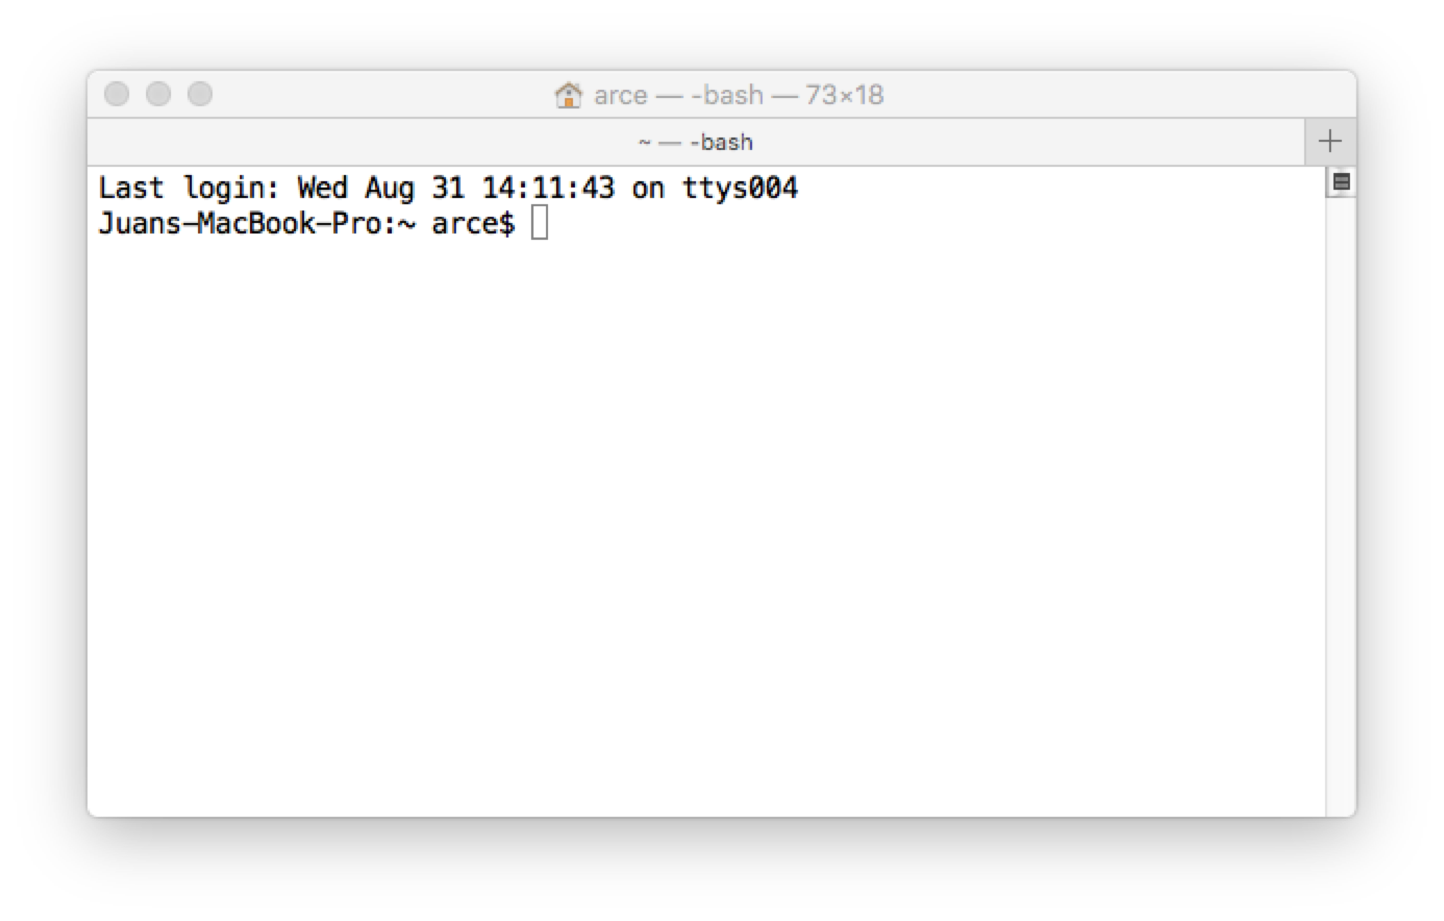
\includegraphics{./figures/terminal-mac.png}
\caption{Terminal window on Mac OS}
\end{figure}

If you are a Linux user then you should be able to start a terminal
without the need for any installation. Terminal on a Linux system
running Ubuntu can be accessed using Ctrl+Alt+T. Multiple tabs can be
opened by hitting Ctrl+Shift+T.

\begin{figure}
\centering
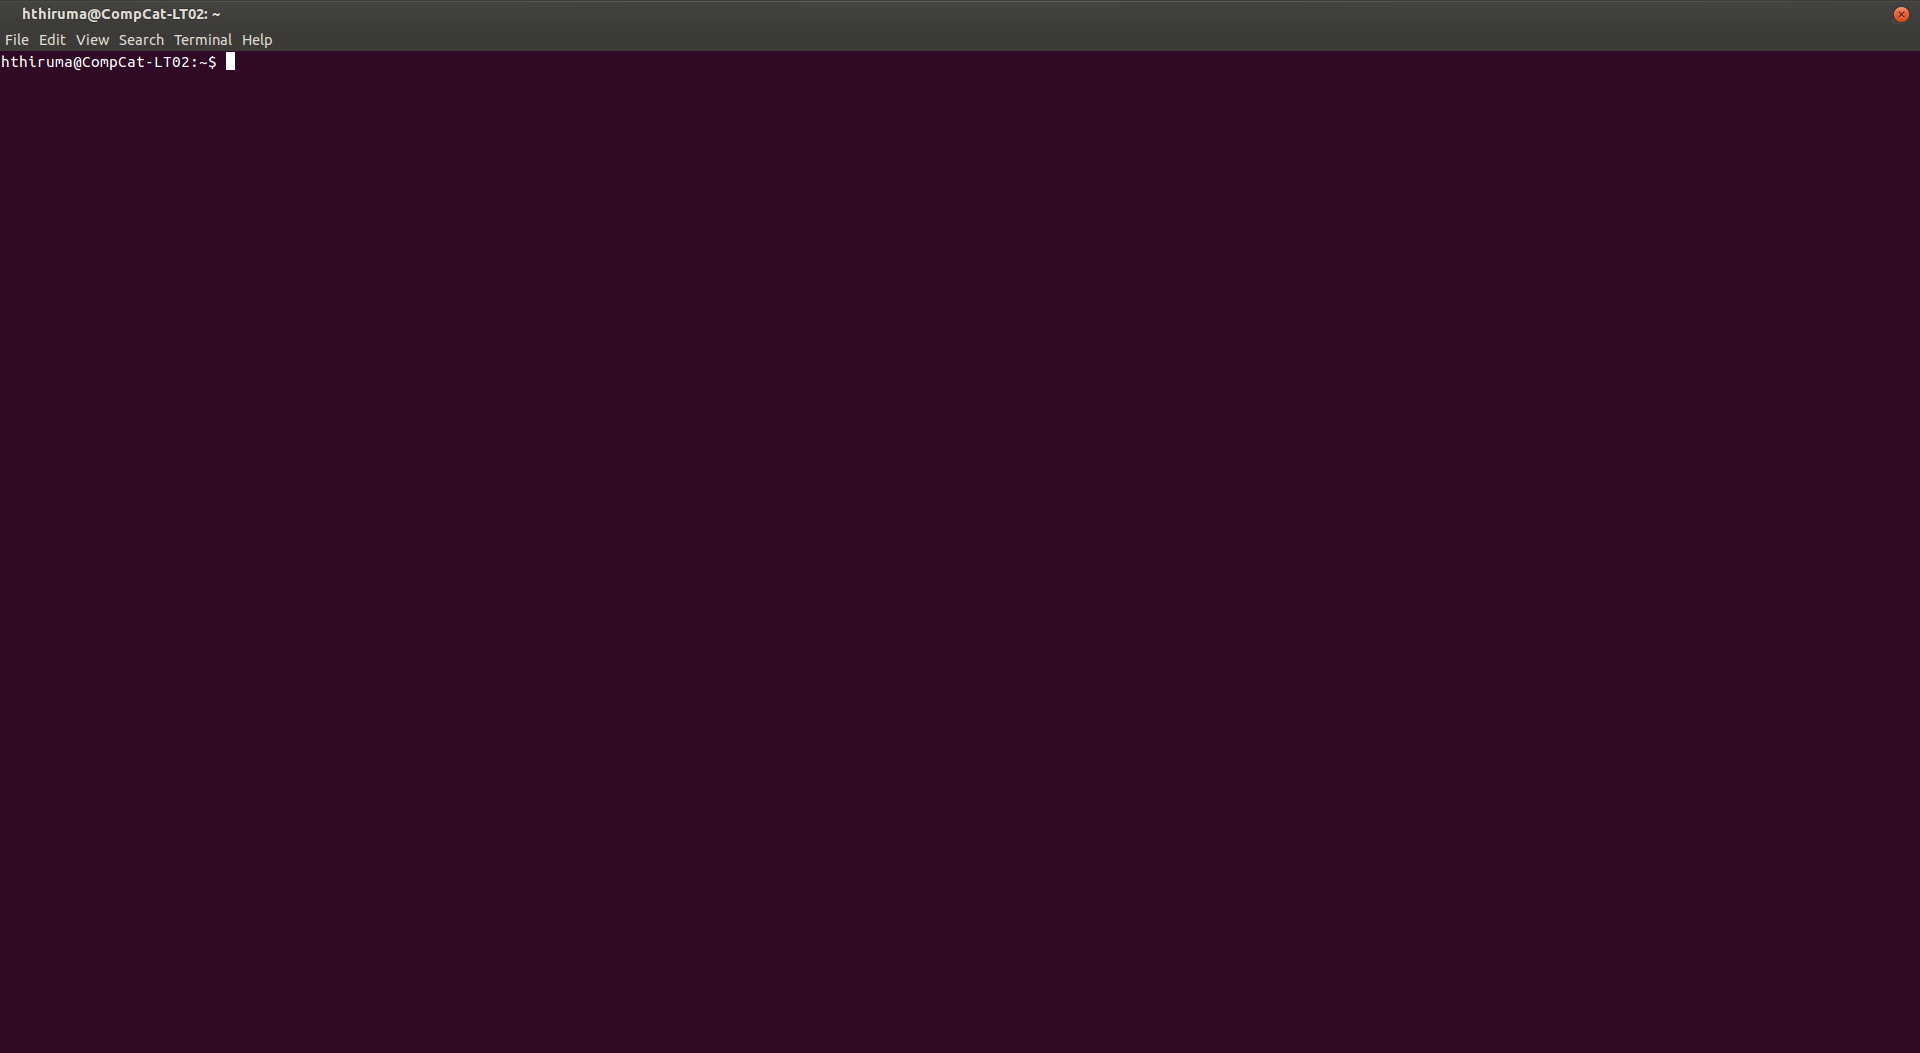
\includegraphics{./figures/Ubuntu-terminal.png}
\caption{Terminal window on Linux}
\end{figure}

Windows users can install either
\href{http://mobaxterm.mobatek.net/}{MobaXTerm} or
\href{http://www.straightrunning.com/XmingNotes/}{Xming}. We recommend
MobaXTerm.

\begin{figure}
\centering
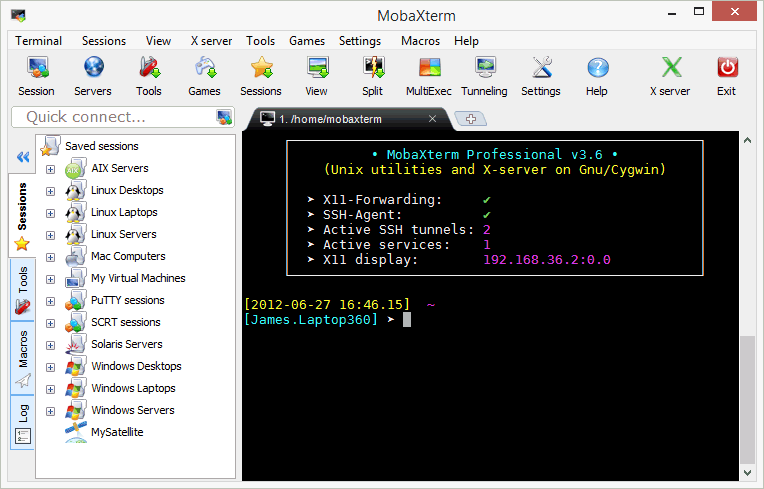
\includegraphics{./figures/moba.png}
\caption{MobaXTerm Terminal window on Windows}
\end{figure}

    \subsubsection{Logging into
clusters/supercomputers}\label{logging-into-clusterssupercomputers}

In order to login into your account in a cluster or supercomputer you
need the address of the remote machine and have an account in it. One
should be able to connect to the remote computer typing the following
command in a terminal

\begin{verbatim}
ssh -X user_name@supercomputer_address
\end{verbatim}

Addresses of the supercomputers used by the group are

\begin{verbatim}
System: colossus
Address: colossus.egr.uh.edu

System: opuntia
Address: opuntia.cacds.uh.edu

System: maxwell 
Address: cusco.hpcc.uh.edu

System: cori
Address: cori.nersc.gov

System: stampede2
Address: stampede2.tacc.utexas.edu

System: uhpc
Address: uhpc.hpcc.uh.edu

System: juniper
Address: juniper.hpcc.uh.edu

System: sabine
Address: sabine.cacds.uh.edu
\end{verbatim}

The environment has to be set up the first time the user logs in to load
all the programs, modules and executables required for efficient
operation. This is addressed in the final section of this chapter.

    \subsubsection{Configuration of a .cshrc
file}\label{configuration-of-a-.cshrc-file}

When the user logs in to a remote machine, there are certain default
parameters and applications that will be enabled when you enter the
terminal. The most common types of shell environments used are
\emph{BASH} shells and \emph{CSH/TCSH} shells. These environments will
have a \emph{.(shell)rc} file associated with it. In almost all
situations, a user must modify the list of programs, defaults and
executables in order to suit his or her needs. This information is
stored in the \emph{.(shell)rc} file in your system. For the clusters on
campus, the defaults are setup with \emph{CSH} shells. This file is
loaded and executed every time you log in into the machine, and can be
modified according to your needs.

The \emph{.cshrc} can be accessed through the \emph{vi} editor by
executing the command

\texttt{vi\ .cshrc}

    This file is unique to the user and contains syntax that configures your
personal profile in the cluster/supercomputer. We do not expect you know
learn these concepts off the bat, but you are ultimately expected to
understand what exactly goes on behind the terminal

A typical \emph{.cshrc} file looks like this:

\begin{verbatim}
module load vasp
module load ase
module load povray

setenv PATH ~/bin:/home/jarceram/apps:${PATH}

setenv DB ~/Dropbox/Post-Doc/workbooks_jmax/databases/

if ! $?PYTHONPATH then
    setenv PYTHONPATH
endif

setenv PYTHONPATH /share/apps/python2.6-extra/lib/python2.6/site-packages:${PYTHONPATH}

setenv VASPDIR '/share/apps/vasp/5.4.1/bin'
setenv VASP_COMMAND '/share/apps/openmpi-1.10.2-intel/bin/mpirun ${VASPDIR}/${VASP_EXEC}'
setenv VASP_PP_PATH /share/apps/vasp/vasp-potentials
\end{verbatim}

    The user must ensure that the enviroment variables that link VASP with
ASE are pointing to correct and accessible locations. Those environment
variables are \emph{VASPDIR}, \emph{VASP\_COMMAND} and
\emph{VASP\_PP\_PATH}.

Also, depending on the cluster or supercomputer you are working on, you
should be able to set helpful environmental variables by loading modules
that were defined by the administrators. This is shown in the first
three lines in the example \emph{.cshrc}.

If you have questions about what your \emph{.cshrc} file should contain,
ask somebody in the lab, he/she will be happy to help you.

    \subsection{Linux}\label{linux}

This document was created as a Jupyter Notebook and inherently cannot
execute shell commands. Therefore, we recommend that the reader copies
these commands onto an actual terminal and execute these commands for
the purposes of practise. Code must be copied, pasted and executed on
the terminal line by line.

\subsubsection{Basic shell commands}\label{basic-shell-commands}

These commands will help you navigate through your folders, copy files,
remove files and some other basic shell commands will be used in the
examples of this section.

\paragraph{Folder creation and
navigation}\label{folder-creation-and-navigation}

Once in your \$HOME directory (\$HOME is the environmental variable that
stores the absolute path to your home directory), create a directory
named "example" and navigate into it. \textbf{mkdir} (create directory)
and \textbf{cd} (change directory) are the commands will be used for
this exercise.

Creating a new directory

\begin{verbatim}
mkdir example
cd example
\end{verbatim}

Creating a new folder structure

\begin{verbatim}
mkdir -p topfolder/nextfolder/nextnextfolder
cd topfolder/nextfolder
\end{verbatim}

To navigate the folder structure, the \texttt{cd} command will be used
once again

\begin{verbatim}
cd ..        # Navigate one level above
cd ../../    # Navigate two levels above
\end{verbatim}

    \paragraph{Displaying contents of files and
folders}\label{displaying-contents-of-files-and-folders}

The \textbf{echo} command allows the user to print the values stored by
environment variables, or in general it can be used as a generic
\textbf{print} statement.

\begin{verbatim}
echo "Hello new member!!!"
echo \$HOME
\end{verbatim}

The output from the command line can be \emph{piped} out to an object
such as a text file. For example

\begin{verbatim}
echo "If you're reading this, your life is going to be miserable, muhahahahah" > greetings.txt
\end{verbatim}

Then, the \textbf{ls} command can be used to list the contents of the
directory in which the user is currently in. In my case, there is a load
of files that are required for building this tutorial. You can also see
the greetings.txt file we just created.

    \begin{Verbatim}[commandchars=\\\{\}]
{\color{incolor}In [{\color{incolor}3}]:} \PY{n}{ls}
\end{Verbatim}


    \begin{Verbatim}[commandchars=\\\{\}]
\textcolor{ansi-red}{Circulating fluidized bed.mp4}* dft\_tutorial.tex
README.md                      dft\_tutorial.toc
\textcolor{ansi-red}{TODO}*                          \textcolor{ansi-blue}{figures}/
\textcolor{ansi-red}{ZrO2\_surface\_101\_ex.traj}*      \textcolor{ansi-red}{for-arce.png}*
\textcolor{ansi-blue}{\_minted-dft\_tutorial}/          greetings.txt
\textcolor{ansi-red}{ase.png}*                       \textcolor{ansi-red}{py\_ex\_data.txt}*
dft\_tutorial.aux               renamed.dat
\textcolor{ansi-red}{dft\_tutorial.html}*             \textcolor{ansi-blue}{test}/
dft\_tutorial.log               \textcolor{ansi-red}{test.png}*
dft\_tutorial.org               tutorial.ipynb
dft\_tutorial.out               tutorial.pdf
dft\_tutorial.pyg

    \end{Verbatim}

    "greetings.txt" is a text file located in your current directory. If you
want to display the content of a typical ASCII text file, you can use
commands such as \textbf{more}, \textbf{less}. The syntax for these
commands is given below

\begin{verbatim}
more <filename>
less <filename>
\end{verbatim}

These commands allow the user the "scroll" through the file if its
contents exceed one window. Scrolling can be achieved by hitting the
space-bar. The commands can be killed by hitting \texttt{q}

Other useful commands for reading files are \textbf{head} and
\textbf{tail}, which display the first 10 lines and the last 10 lines of
a file, respectively.

\begin{verbatim}
head POSCAR               # Displays first 10 lines in file
tail POSCAR               # Displays last 10 lines in file
\end{verbatim}

Arguments can be passed to these commands to display more lines than the
default number. This is done as follows

\begin{verbatim}
head -n 71 POSCAR               # Displays first 71 lines in file
tail -n 19 POSCAR               # Displays last 19 lines in file
\end{verbatim}

    \paragraph{Manipulating contents of files and
folders}\label{manipulating-contents-of-files-and-folders}

\subparagraph{Piping and Appending}\label{piping-and-appending}

The previous section showed how terminal output could be piped to a file
using the \texttt{\textgreater{}} symbol. Another way of piping output
into a file is

\texttt{command\ \textgreater{}\ output.txt\ \ \ \ \ \ \ \#\ All\ the\ output\ from\ executing\ the\ command\ is\ piped\ into\ output.txt}

This command essentially creates a new file "output.txt" and inserts the
text into it. If a file of the same name exists, then all the contents
in the file are overwritten.

However, if the user would like to append text to an existing file, then
they can use
\texttt{command\ \textgreater{}\textgreater{}\ output.txt"}. Using
\texttt{\textgreater{}} will again erase the original content of the
tect file. For example

\begin{verbatim}
echo "This is the second line" >> hello.txt
\end{verbatim}

Reading the contents of \texttt{output.txt} should give you
\texttt{If\ you\textquotesingle{}re\ reading\ this,\ your\ life\ is\ going\ to\ be\ miserable,\ muhahahahah\ This\ is\ the\ second\ line}

    \subparagraph{Copy, move and delete files and
folders}\label{copy-move-and-delete-files-and-folders}

Remove, copy files, move or renanme files are tasks that are very often
used when working with a terminal to explore and manipulate data files.
Lets continue with the tutorial with these code lines in order to show
you how they work.

Lets start with renaming the file you just created before "hello.txt".
We will use the "\emph{=mv=}" command to show the two main uses of this
function. The first use we will show here is as rename command.
\#+BEGIN\_SRC sh mv hello.txt renamed.dat ls \#+END\_SRC

Remember that with "\emph{=ls=}" command we are showing the content of
the current folder. You should see now a "rename.dat" file in your
current position. \#+RESULTS: : renamed.dat

To move a file from one folder to another we will first create a folder
called test, and move the file "renamed.dat" into that folder.
\#+BEGIN\_SRC sh \# This creates a file renamed.dat touch renamed.dat

mkdir test mv renamed.dat test/

ls test \#+END\_SRC

\section{+RESULTS:}\label{results}

: renamed.dat

A file or folder may be copied and pasted into another file or folder of
the same name, or different name using the \emph{=cp=} command. Let us
demonstrate how this can be done by copying the file "renamed.dat", from
the folder \emph{test} and into the current directory. \#+BEGIN\_SRC sh
\# Copies the file renamed.dat from test/ to the current directory (.)
cp test/renamed.dat . ls \#+END\_SRC

\section{+RESULTS:}\label{results-1}

\section{+begin\_example}\label{begin_example}

\section{dft\_tutorial.org}\label{dft_tutorial.org}

Icon dft\_tutorial (Copia en conflicto de Juan Manuel Arce
2016-09-01).org dft\_tutorial (Juan Manuel Arce's conflicted copy
2016-09-07).org dft\_tutorial.html dft\_tutorial.org figures
py\_ex\_data.txt renamed.dat test \#+end\_example

It is also possible to copy an entire folder by using the \emph{=cp=}
command recursively. To use a command recursively, you must pass the
argument =-r= along with the command. The usage of recursive copying is
demonstrated below. We will try to copy the entire folder test and
create another folder test-1 with the same contents \#+BEGIN\_SRC sh cp
-r test test-1 ls test ls test-1 \#+END\_SRC

\section{+RESULTS:}\label{results-2}

\begin{description}
\tightlist
\item[: renamed.dat]
renamed.dat
\end{description}

To remove a file or a folder, one should use the \emph{=rm=} command as
\#+BEGIN\_SRC sh \# List contents before deletion ls test-1

\section{Remove renamed.dat from
test-1}\label{remove-renamed.dat-from-test-1}

rm test-1/renamed.dat

echo "Deleted"

\section{List contents after
deletion}\label{list-contents-after-deletion}

ls test-1

\section{Remove test-1 folder}\label{remove-test-1-folder}

\section{List contents of current
directory}\label{list-contents-of-current-directory}

ls

rm -r test-1

\section{List contents of current directory after
deletion}\label{list-contents-of-current-directory-after-deletion}

ls

\section{+END\_SRC}\label{end_src}

\section{+RESULTS:}\label{results-3}

\section{+begin\_example}\label{begin_example-1}

\section{dft\_tutorial.org}\label{dft_tutorial.org-1}

Icon dft\_tutorial (Copia en conflicto de Juan Manuel Arce
2016-09-01).org dft\_tutorial (Juan Manuel Arce's conflicted copy
2016-09-07).org dft\_tutorial.html dft\_tutorial.org figures
py\_ex\_data.txt renamed.dat test test-1

\section{dft\_tutorial.org}\label{dft_tutorial.org-2}

Icon dft\_tutorial (Copia en conflicto de Juan Manuel Arce
2016-09-01).org dft\_tutorial (Juan Manuel Arce's conflicted copy
2016-09-07).org dft\_tutorial.html dft\_tutorial.org figures
py\_ex\_data.txt renamed.dat test \#+end\_example

**** Text editors VI Editor and Emacs are commonly used text editors in
the world of computing. They are similar to something familiar like
Notepad in windows. Text editors are extremely important because they
can open any file the contains normal ASCII text. These files can be
anything from configuration files to scripts. They are very lightweight
and are extremely versatile. Both editors are fairly difficult to work
with at first, and possess a steep learning curve. They are useful for
different purposes, and it is best to know the basics of both, to ensure
a smooth manner of working. Outside of standard tutorials, we strongly
encourage you to look up resources on the internet. It has always
happened that we learn something new with every new Google search. *****
VI Editor vi editor is a very powerful and handy text editor used
commonly by members in the group. The best way one can learn this editor
is to go through the VIM Tutorial. This can be accessed on any terminal
by typing \#+BEGIN\_SRC sh vimtutor \#+END\_SRC

\section{+RESULTS:}\label{results-4}

\section{+BEGIN\_EXAMPLE}\label{begin_example-2}

\section{= W e l c o m e t o t h e V I M T u t o r - Version 1.7
=}\label{w-e-l-c-o-m-e-t-o-t-h-e-v-i-m-t-u-t-o-r---version-1.7}

\begin{verbatim}
 Vim is a very powerful editor that has many commands, too many to
 explain in a tutor such as this.  This tutor is designed to describe
 enough of the commands that you will be able to easily use Vim as
 an all-purpose editor.

 The approximate time required to complete the tutor is 25-30 minutes,
 depending upon how much time is spent with experimentation.
\end{verbatim}

\section{+END\_EXAMPLE}\label{end_example}

***** Emacs Emacs is again a very powerful and versatile text editor,
used by some members (Juan Manuel and Hari) in the group. Emacs can be
accessed by typing =emacs= in the terminal. In most systems, the emacs
that pops up is one built into the command line, in a manner similar to
the VI editor. The version of emacs used by us in the group has a
graphical user interface associated with it, as well as many useful
packages and functions built in. This emacs is intuitively called jmax,
also the work of John Kitchin. Emacs can be learned by opening it and
accessing its tutorial on the main page.

\section{+BEGIN\_SRC sh}\label{begin_src-sh}

emacs \#+END\_SRC

\section{+RESULTS:}\label{results-5}

\section{+attr\_org: :width 200}\label{attr_org-width-200}

\section{+attr\_html: :width 600px}\label{attr_html-width-600px}

\section{+caption: Emacs GUI}\label{caption-emacs-gui}

{[}{[}./figures/emacs.png{]}{]}

** Python *** Introduction Python is a programming language which is
used and documented extensively in scientific programming. We use python
to interface with the Atomic Simulation Environment (ASE), which is used
to build, setup and modify molecular models. One of the best resources
for learning scientific python is through
{[}{[}http://www.scipy-lectures.org/{]}{[}SciPy{]}{]}, which has
extensive notes and examples on using python.
{[}{[}http://kitchingroup.cheme.cmu.edu/pycse/pycse.html{]}{[}PYCSE{]}{]}
is a module written by
{[}{[}http://kitchingroup.cheme.cmu.edu/{]}{[}John Kitchin{]}{]} and has
many examples which use standard Python Modules, as well as custom
modules in PYCSE. We recommend that you practise these examples as much
as possible, to get a good understanding of python and how to use it to
suit your needs. *** Common used commands and basics Even though it is
impossible to be thorough in explaining in detail all commands and
functions, we will show some of the most common commands and functions
that you will more likely see in python scripts used for some of us in
the lab. Again, we encourage you to review the broad documentation in
the official webpage of
{[}{[}https://docs.python.org/2/{]}{[}Python{]}{]}.

In order to test the commands and functions you should intialize a
python interpreter, with the command "python" in a linux terminal while
in a computer with Python installed in it. **** Print \#+BEGIN\_SRC
python print 'Hello, this is a sample sentence!' print
'This\tis\ttab\tseparated\ttext' \#+END\_SRC

\section{+RESULTS:}\label{results-6}

\begin{description}
\tightlist
\item[: Hello, this is a sample sentence!]
This is tab separated text
\end{description}

**** Arrays and Dictionaries \#+BEGIN\_SRC python import numpy as np

\section{Array with a range of numbers from 0 to 5, with step size of
1.}\label{array-with-a-range-of-numbers-from-0-to-5-with-step-size-of-1.}

\section{Here, the end point is not
included.}\label{here-the-end-point-is-not-included.}

a = np.arange(0, 5, 1) print a

\section{Dictionary with keys and corresponding values showing date
format}\label{dictionary-with-keys-and-corresponding-values-showing-date-format}

b = \{'Day': 'DD', 'Month': 'MM', 'Year': 'YYYY'\}

print b print b{[}'Month'{]} \#+END\_SRC

\section{+RESULTS:}\label{results-7}

\begin{description}
\tightlist
\item[: {[}0 1 2 3 4{]}]
\{'Year': 'YYYY', 'Day': 'DD', 'Month': 'MM'\}

MM
\end{description}

**** Variable definition In this section we will define 4 types of
variables: string variables, scalar variables (either integer or float
numbers), vector or 1-D array and matrix or 2-D array. \#+BEGIN\_SRC
python string = 'sample text' scalar = 12 array\_1d =
{[}1,3,6,-4,0.95{]} array\_2d = {[}{[}1,2{]},{[}-3,2.0{]}{]}

print string print scalar print array\_1d print array\_2d \#+END\_SRC

\section{+RESULTS:}\label{results-8}

\begin{description}
\tightlist
\item[: sample text]
12

{[}1, 3, 6, -4, 0.95{]}

{[}{[}1, 2{]}, {[}-3, 2.0{]}{]}
\end{description}

*** Loading python modules and functions In order to use not pre-loaded
commands or functions in python you need to load them first from their
modules. This means that by default Python has loaded a set of modules
which contains the commands or functions that you can use right away,
however, if you want to use a function that is not pre-loaded then you
need to load it from the corresponding module.

Probably the most common modules that you are going to use are these:
\textbar{} module \textbar{} example functions \textbar{} Description
\textbar{}
\textbar{}-\/-\/-\/-\/-\/-\/-\/-\/-\/-\/-\/-\/-\/-\/-\/-\/-+-\/-\/-\/-\/-\/-\/-\/-\/-\/-\/-\/-\/-\/-\/-\/-\/-\/-\/-\/-\/-\/-\/-\/-\/-\/-\/-\/-\/-\/-+-\/-\/-\/-\/-\/-\/-\/-\/-\/-\/-\/-\/-\/-\/-\/-\/-\/-\/-\/-\/-\/-\/-\/-\/-\/-\/-\/-\/-\/-\/-\/-\/-\/-\/-\/-\/-\/-\/-\/-\/-\/-\/-\/-\/-\/-\/-\/-\/-\/-\/-\/-\/-\/-\/-\/-\/-\textbar{}
\textbar{} os \textbar{} mkdir, remove, getcwd, chdir \textbar{} module
to access operative system functionality \textbar{} \textbar{} ase
\textbar{} Atoms \textbar{} useful to handle atomic objects \textbar{}
\textbar{} ase.io \textbar{} read, write \textbar{} used to load and
write atomic objects \textbar{} \textbar{} ase.calculators \textbar{}
Vasp, Abinit \textbar{} take atomic objects and calculate energies,
forces, etc \textbar{} \textbar{} \textbar{} \textbar{} \textbar{}

Modules are loaded as follows \#+BEGIN\_SRC python import os from ase
import Atoms from ase.io import read from ase.calculators.vasp import
Vasp \#+END\_SRC

\section{+RESULTS:}\label{results-9}

*** Simple data manipulation example Data extraction and manipulation is
an activity that become important, specially when dealing with huge data
files or when automatization is required in order to post-process the
data in an efficient way.

Lets consider that you want to determine the value of the lattice
parameter of a bulk structure that minimizes the energy of the system.
Do not worry to much right now in the details behind this. One approach
to determine that is determining the energy of the system while changing
the value of the lattice constant and then fitting the data to an
equation to obtain the value that minimizes the energy. For now, we will
focus in using python to extract data and manipulate them to create a
simple plot. We will explain later how to determine these data points
with a valid set up.

Create a text file using \emph{vi} called py\_ex\_data.txt and copy all
lines. Note that data columns are separated by tabs. \#+BEGIN\_SRC sh
3.8 -12.28653631 3.85 -12.65124072 3.9 -12.88611724 3.95 -13.01158939 4
-13.04446413 4.05 -12.99864981 4.1 -12.88660177 4.15 -12.71939621 4.2
-12.5064955 \#+END\_SRC

\section{+BEGIN\_SRC sh :exports none}\label{begin_src-sh-exports-none}

\section{Create file with data mentioned
above}\label{create-file-with-data-mentioned-above}

cat \textgreater{} py\_ex\_data.txt \textless{}\textless{} EOF 3.8
-12.28653631 3.85 -12.65124072 3.9 -12.88611724 3.95 -13.01158939 4
-13.04446413 4.05 -12.99864981 4.1 -12.88660177 4.15 -12.71939621 4.2
-12.5064955 EOF \#+END\_SRC

A simple code to read this file and extract the datapoints could look
like the following: \#+BEGIN\_SRC python import matplotlib.pyplot as plt

\section{This is only a comment.}\label{this-is-only-a-comment.}

\section{Reading data file.}\label{reading-data-file.}

data = open('py\_ex\_data.txt','r') lines = data.readlines() a = {[}{]}
e = {[}{]} \# To go through all lines we conveniently use a FOR loop for
line in lines: values = line.split() a.append(values{[}0{]})
e.append(values{[}1{]})

print a print e plt.plot(a,e,'s:k') plt.show()\\
\#+END\_SRC

\section{+RESULTS:}\label{results-10}

\begin{description}
\tightlist
\item[: {[}'3.8', '3.85', '3.9', '3.95', '4', '4.05', '4.1', '4.15',
'4.2'{]}]
{[}'-12.28653631', '-12.65124072', '-12.88611724', '-13.01158939',
'-13.04446413', '-12.99864981', '-12.88660177', '-12.71939621',
'-12.5064955'{]}
\end{description}

Look at the four last lines, we want to display whatever were saved in
the variables \emph{a} and \emph{e}, and we used pyplot to generate a
graph with those datapoints. The resulting plot should look like the
following:

\section{+attr\_org: :width 200}\label{attr_org-width-200-1}

\section{+attr\_html: :width 400px}\label{attr_html-width-400px}

\section{+caption: Example plot}\label{caption-example-plot}

{[}{[}./figures/py\_ex\_data.png{]}{]}

** Atomic Simulation Environment (ASE) ASE is an Atomic Simulation
Environment written in the Python programming language with the aim of
setting up, steering, and analyzing atomistic simulations (adapted from
{[}{[}https://wiki.fysik.dtu.dk/ase/about.html{]}{[}ASE{]}{]}). The ASE
has been constructed with a number of ``design goals'' that make it:

\begin{itemize}
\item
  Easy to use: Setting up an atomistic total energy calculation or
  molecular dynamics simulation with ASE is simple and straightforward.
  ASE can be used via a graphical user interface, Command line tools and
  the Python language. Python scripts are easy to follow (see What is
  Python? for a short introduction). It is simple for new users to get
  access to all of the functionality of ASE.
\item
  Flexible: Since ASE is based on the Python scripting language it is
  possible to perform very complicated simulation tasks without any code
  modifications. For example, a sequence of calculations may be
  performed with the use of simple ``for-loop'' constructions. There
  exist ASE modules for performing many standard simulation tasks.
\item
  Customizable: The Python code in ASE is structured in modules intended
  for different purposes. There are ase.calculators for calculating
  energies, forces and stresses, ase.md and ase.optimize modules for
  controlling the motion of atoms, constraints objects and filters for
  performing nudged-elastic-band calculations etc. The modularity of the
  object-oriented code make it simple to contribute new functionality to
  ASE.
\item
  Pythonic: It fits nicely into the rest of the Python world with use of
  the popular NumPy package for numerical work (see Numeric arrays in
  Python for a short introduction). The use of the Python language
  allows ASE to be used both interactively as well as in scripts.
\end{itemize}

**** Installing ASE ASE is a bundle of python modules which can be
invoked or loaded when atomic simulations are required to be set up or
analyzed. The easiest way of installing ase, is to download the latest
source tar ball from the website. Once downloaded, the tar ball must be
extracted, and installation can be completed by running

\section{+BEGIN\_SRC sh}\label{begin_src-sh-1}

python setup.py install -\/-user \#+END\_SRC

Sometimes, it is necessary to add the installation path in your
\emph{=.cshrc=} file and add \textasciitilde{}/.local/bin to the front
of your PATH environment variable. This is dependent on the system you
are using.

**** Reading and Viewing simple atoms files We have downloaded a
standard =cif= file (Crystallographic Information Format) from the
International Zeolite Website
{[}{[}http://www.iza-online.org/{]}{[}IZA{]}{]} as an example structure.
The =cif= file is present as MFI.cif in this folder. The ASE module
=ase.io= has the functions read and write which are capable of handling
various formats for atomic structure, and can be used to set up every
forseeable future =Vasp= calculation. An example of how to read a =cif=
file is shown in the code block below.

\section{+BEGIN\_SRC python}\label{begin_src-python}

\section{Import the read and write functions from the ase.io
module.}\label{import-the-read-and-write-functions-from-the-ase.io-module.}

from ase.io import read, write

\section{Import the visualize function to view the imported atoms
object.}\label{import-the-visualize-function-to-view-the-imported-atoms-object.}

from ase.visualize import view

\section{Load the cif file into a pythonic object called
'atoms'.}\label{load-the-cif-file-into-a-pythonic-object-called-atoms.}

atoms = read('MFI.cif')

\section{View the 'atoms' object.}\label{view-the-atoms-object.}

view(atoms) \#+END\_SRC

Note: This jmax interface becomes inactive when you call the view
function. To make it active again, close the view pop-up and then hit
Ctrl+g.

=Vasp= calculations require a certain set of input files for calculation
initialization. One of these files pertains to the initial structure and
cartesian coordinates of the model under investigation. The name of this
file is =POSCAR=. One can simply read a =cif= and write out a =POSCAR=
using the functions provided by the ase.io module. An example of writing
files of various formats is shown below

\section{+BEGIN\_SRC python}\label{begin_src-python-1}

from ase.io import read, write

atoms = read('MFI.cif')

\section{Write the cartesian coordinates file in the =vasp= POSCAR
format.}\label{write-the-cartesian-coordinates-file-in-the-vasp-poscar-format.}

\section{File written in the folder
'images'}\label{file-written-in-the-folder-images}

write('images/POSCAR\_ZSM-5', atoms, format='vasp')

\section{Write the cartesian coordinates file in the =xyz=
format}\label{write-the-cartesian-coordinates-file-in-the-xyz-format}

write('images/atoms\_xyz', atoms, format='xyz') \#+END\_SRC

\section{+RESULTS:}\label{results-11}

**** Building gas phase molecules Smaller models involving gas phase
molecules and systems on simple surfaces are usually built up from
scratch, using the modules and functions availble in ase. This can
either be done through scripting or through the =ase-gui= interface.
Extensive documentation on using the =ase-gui= can be accessed on the
ASE website at
{[}{[}https://wiki.fysik.dtu.dk/ase/ase/gui/gui.html{]}{[}Link{]}{]}.
Here, we will provide a quick introduction on creating different
systems.

The most simple demonstration to begin with, would be to model a simple
gas phase molecule such as H\_\{2\}O. ASE provides a number of ways to
build and modify models, and we will explore two ways. 1) using python
scripting and 2) using the ASE Graphical user interface. We recommend
that you use scripting wherever possible as this keeps track of all
changes made to the model, whenever documentation is necessary.

Gas phase models are the simplest models to make, and are the least
expesive in terms of computational processing time. Such systems require
that they are enclosed in a vacuum cell of certain dimensions, depending
on the size of the model itself. The presence and size of this cell
ensures that when DFT calculations are performed, and periodic boundary
conditions are implemented in X, Y and Z directions, there is minimal
interaction energy between the models. Hence, one should perform
calculations to ensure that energies and cell sizes are well converged,
before proceeding to use data from these calculations. We will build a
simple H2O molecule in a box of 10 x 10 x 10 \AA.

Note: ase.structure may have been updated to a newer version, depending
on your version of ase. \#+BEGIN\_SRC python from ase.structure import
molecule from ase.visualize import view

atoms = molecule('H2O') atoms.set\_cell({[}10, 10, 10{]}) atoms.center()

view(atoms) \#+END\_SRC

\section{+attr\_org: :width 100}\label{attr_org-width-100}

\section{+attr\_html: :width 400px}\label{attr_html-width-400px-1}

\section{+caption: H\_\{2\}O molecule in a
box}\label{caption-h_2o-molecule-in-a-box}

{[}{[}./figures/molec\_h2o\_ase\_ex.png{]}{]}

As you can see we have used the "molecule" and "view" functions from the
"structure" and "visualize" subpackages in order to build and visualize
the molecule. Again, you need to load modules and subpackages in order
to use installed/non-default python packages.

\section{+BEGIN\_SRC python}\label{begin_src-python-2}

\section{From the Atoms and Atom
modules}\label{from-the-atoms-and-atom-modules}

from ase import Atom, Atoms from ase.visualize import view from ase.io
import read, write

\section{Creating a random model with H, O and C at random
positions}\label{creating-a-random-model-with-h-o-and-c-at-random-positions}

atoms = Atoms({[}Atom('H', {[}0, 0, 0{]}), Atom('O', {[}1, 1, 1{]}),
Atom('C', {[}2, 2, 1{]}){]})

\section{\texorpdfstring{Set a cell of dimensions 10 \AA
atoms.set\_cell({[}10, 10,
10{]})}{Set a cell of dimensions 10 atoms.set\_cell({[}10, 10, 10{]})}}\label{set-a-cell-of-dimensions-10-atoms.set_cell10-10-10}

write('images/not-centered.png', atoms, show\_unit\_cell=True) \# The
atoms and the cell originate at {[}0, 0, 0{]}, and the model will not be
centered within the cell \# it is important to center the model so that
there is equal vacuum on all sides. atoms.center()

write('images/centered.png', atoms, show\_unit\_cell=True)
write('images/POSCAR\_random', atoms, format='vasp') \#+END\_SRC

**** Building crystal structures Crystals are materials that maintain an
order in a microscopic scale and in all three dimensions. In other
words, the building block (unit cell) of a crystalline material is
repeated in the 3-dimensional space, or it is isotropic. Take for
instance the example shown in the following figure in which we are
displaying the structure of the rutile crystal phase of TiO\_\{2\}
(rut-TiO\_\{2\}). In this figure, the dashed-line box represent the
limits of the unit cell that is repeated in all directions.

\section{+attr\_html: :width 600px}\label{attr_html-width-600px-1}

\section{+caption: Crystal structure of
rutile-TiO\_\{2\}}\label{caption-crystal-structure-of-rutile-tio_2}

{[}{[}./figures/rut-TiO2\_ex.png{]}{]}

One way to build a crystal structure through ASE is the "spacegroup"
subpackage. This subpackage requires that you to provide the crystal
space group, the lattice parameters and the scaled positions of the
unique atoms (the number of atoms provided not necessarily match with
the number of atoms in the unit cell). Lets continue with the example of
rut-TiO\_\{2\} and try to build the same crystal structure. We will need
detailed information about this crystal that can be found in scientific
articles or databases. An example of python script to carry out the task
can look like the following:

\section{+BEGIN\_SRC python}\label{begin_src-python-3}

from ase.lattice.spacegroup import crystal from ase.visualize import
view

\section{Lattice parameters. Experimetnal values for TiO2
rutile}\label{lattice-parameters.-experimetnal-values-for-tio2-rutile}

a = 4.5937 c = 2.9587

\section{Using the 'crystal' function from 'spacegroup'
subpackage}\label{using-the-crystal-function-from-spacegroup-subpackage}

\section{Data provided (in order of
appearence)}\label{data-provided-in-order-of-appearence}

\section{Unique atoms in unit cell; scaled positions of unique
atoms;}\label{unique-atoms-in-unit-cell-scaled-positions-of-unique-atoms}

\section{Space group ID \#; dimension of unit cell (lattice param. and
angles)}\label{space-group-id-dimension-of-unit-cell-lattice-param.-and-angles}

rut = crystal({[}'Ti','O'{]},
basis={[}(0.0,0.0,0.0),(0.3048,0.3048,0.0){]}, spacegroup=136,
cellpar={[}a, a, c, 90, 90, 90{]})

view(rut) \#+END\_SRC

\section{+attr\_html: :width 300px}\label{attr_html-width-300px}

\section{+caption: Output after running the previous python script that
builds
rut-TiO\_\{2\}}\label{caption-output-after-running-the-previous-python-script-that-builds-rut-tio_2}

{[}{[}./figures/rut-TiO2\_ase\_ex.png{]}{]}

As you can see from what was displayed through ASE graphical user
interface, the unit cell of rut-TiO\_\{2\} contains two Ti and four O
atoms, however, we only specified two positions in the script. This is
why we need to provide the space group, in order to let know ASE where
the other equivalent atoms should be placed according to symmetric
positions that are dependent of the space group.

Even though you can provide of very reliable experimental information,
the atomic positions and cell size and shape usually need to be
computationally optimized before can be used to generate a surface or
for energy comparisons. We will talk later about a method that can be
used to optimize a crystal structure.

**** Building surfaces If you want to simulate the adsorption of a
chemical compounds and its interaction with a solid catalyst, you might
want to create a representative model of the solid in question. Here, we
explain how to create a surface model that could be used for following
calculations, such adsorption tests.

We will build a slab of the (101) exposed facet of tetragonal zirconium
oxide from its crystal structure parameters. First, you will need the
lattice parameters required to build a bulk crystal (as was done for
rut-TiO2 above). The lattice parameters are shown in the piece of code
below, together with an extra line with the function "surface" that can
be used to build a surface from a bulk crystal model. In this case, the
function needs a atoms object ("atoms", here in the code), the plane at
which the cut should be done, the number of layers that should be
included and the length of the vacuum layer in each side of slab (in
angstroms).

\section{+BEGIN\_SRC python}\label{begin_src-python-4}

from ase.lattice.spacegroup import crystal from ase.visualize import
view from ase.lattice.surface import surface

a = 3.63 c = 5.25 z = 0.05

atoms = crystal({[}'Zr', 'O'{]}, basis={[}(0.0, 0.0, 0.0), (0.0, 0.5,
z+0.25){]}, spacegroup=137, cellpar={[}a, a, c, 90, 90, 90{]})

surface = surface(atoms, (1,0,1), 5, 7.5) view(surface) \#+END\_SRC

\section{+attr\_html: :width 200px}\label{attr_html-width-200px}

\section{+caption: Slab of t-ZrO2 (101) built from
bulk.}\label{caption-slab-of-t-zro2-101-built-from-bulk.}

{[}{[}./figures/ZrO2\_surf\_ex.png{]}{]}

Even though this procedure is very simple, one needs to be really
careful in the selection of the surface termination. For instance, by
looking at the slab generated by ASE one can see that the exposed
surface in +z direction has a oxygen termination, that might not be (and
is not) the most stable termination. However, by deleting this "extra"
oxygen atoms on top, we are also changing the Zr/O ratio. The surface
slab is now no longer stoichiometric (Zr\_\{10\}O\_\{18\} instead of
Zr\_\{10\}O\_\{20\}). Is usually a good idea to keep the stoichiometry
in order to avoid strong polarization (\#\#is this right??). This is
usually not a problem for simple metal surfaces that are highly
symetrical or are built by only one distinguishable metal.

One way to solve this problem can be creating a slab with an extra layer
and then deleting the atoms that are not longer needed in order to
maintain the desirable number of layers. At the end, is possible that we
need to shift the position of all atoms in the cell in order to keep the
center of mass in the center of the cell. We are going to use a similar
script to create a slab with an extra layer and then delete some of the
atoms, so we keep only 5 layers in total.

\section{+BEGIN\_SRC python}\label{begin_src-python-5}

from ase.lattice.spacegroup import crystal from ase.visualize import
view from ase.lattice.surface import surface

a = 3.63 c = 5.25 z = 0.05

atoms = crystal({[}'Zr', 'O'{]}, basis={[}(0.0, 0.0, 0.0), (0.0, 0.5,
z+0.25){]}, spacegroup=137, cellpar={[}a, a, c, 90, 90, 90{]})

surface = surface(atoms, (1,0,1), 6, 7.5)

\section{Lets remove the atoms that should lead to a 5-layered
non-oxygen terminated stoichiometric
surface}\label{lets-remove-the-atoms-that-should-lead-to-a-5-layered-non-oxygen-terminated-stoichiometric-surface}

ind2remove = {[}0,1,2,5,33,34{]} for i in sorted(ind2remove,
reverse=True): del surface{[}i{]}

\section{Tranlate atoms to the new
center}\label{tranlate-atoms-to-the-new-center}

cell = surface.get\_cell() com = surface.get\_center\_of\_mass()
surface.translate({[}0,0,0.5*cell{[}2,2{]} - com{[}2{]}{]})

view(surface) \#+END\_SRC

As a result, you should get a new slab with the right termination but
also one that keeps the Zr/O ratio to 1/2. As you can see in the script
we have removed some of the atoms (indicating their indixes in the
atomic object) and we shift the position of the whole slab in the
z-direction so the center of mass of the slab resides again in the
center of the cell.

We now can use this slab for following calculations.

**** Get details of an atoms object ASE has many useful functions, which
when used efficiently are very powerful in automating scripts and
workflow. Given that we have already learned to build complex models and
structures, we must also know how to extract details from atoms objects,
in the case of analysis and post-processing. Examples of simple ase
functions for this purpose are shown below. \#+BEGIN\_SRC python from
ase.io import read

\section{Read atoms from previously stored
POSCAR}\label{read-atoms-from-previously-stored-poscar}

atoms = read('images/POSCAR\_ZSM-5')

\section{Get unit cell parameters}\label{get-unit-cell-parameters}

cell = atoms.get\_cell() print 'Unit cell array:' print cell, '\n'

\section{Get details of all individual atoms making up the entire atoms
object}\label{get-details-of-all-individual-atoms-making-up-the-entire-atoms-object}

\section{Printing only first 10 atom details, using python list
indexing}\label{printing-only-first-10-atom-details-using-python-list-indexing}

print('Details of 10 individual atoms: ') for atom in atoms{[}0:10{]}:
print atom

\section{Get positions of atoms, and print specific
details}\label{get-positions-of-atoms-and-print-specific-details}

positions = atoms.get\_positions()

\section{Using python string formatting and enumeration
concepts}\label{using-python-string-formatting-and-enumeration-concepts}

print('\nAtom specific details: ') for i, atom in
enumerate(atoms{[}0:10{]}): print('Index: \{0\}, Element: \{1\},
Coordinates: \{2\}'.format(i, atom.symbol, positions{[}i{]}))
\#+END\_SRC

\section{+RESULTS:}\label{results-12}

\section{+begin\_src sh}\label{begin_src-sh-2}

Unit cell array: {[}{[} 2.00900000e+01 0.00000000e+00
0.00000000e+00{]}{[} 1.20000000e-15 1.97380000e+01 0.00000000e+00{]} {[}
8.00000000e-16 8.00000000e-16 1.31420000e+01{]}{]}

Details of 10 individual atoms: Atom('O', {[}10.069108,
1.3796862000000008, 9.2230555999999986{]}, index=0) Atom('O',
{[}20.065892000000002, 11.2486862, 2.6520555999999997{]}, index=1)
Atom('O', {[}10.069108, 8.4893137999999997, 9.2230555999999986{]},
index=2) Atom('O', {[}20.065892000000002, 18.358313800000001,
2.6520555999999997{]}, index=3) Atom('O', {[}10.020892000000002,
18.358313800000001, 3.9189444{]}, index=4) Atom('O',
{[}0.024107999999998499, 8.4893137999999997, 10.489944400000001{]},
index=5) Atom('O', {[}10.020892, 11.2486862, 3.9189444{]}, index=6)
Atom('O', {[}0.0241079999999981, 1.3796862000000008,
10.489944400000001{]}, index=7) Atom('O', {[}7.7848750000000013,
1.4665334000000008, 10.5241136{]}, index=8) Atom('O',
{[}2.2601250000000013, 11.335533400000001, 3.9531135999999991{]},
index=9)

Atom specific details: Index: 0, Element: O, Position: {[} 10.069108
1.3796862 9.2230556{]} Index: 1, Element: O, Position: {[} 20.065892
11.2486862 2.6520556{]} Index: 2, Element: O, Position: {[} 10.069108
8.4893138 9.2230556{]} Index: 3, Element: O, Position: {[} 20.065892
18.3583138 2.6520556{]} Index: 4, Element: O, Position: {[} 10.020892
18.3583138 3.9189444{]} Index: 5, Element: O, Position: {[} 0.024108
8.4893138 10.4899444{]} Index: 6, Element: O, Position: {[} 10.020892
11.2486862 3.9189444{]} Index: 7, Element: O, Position: {[} 0.024108
1.3796862 10.4899444{]} Index: 8, Element: O, Position: {[} 7.784875
1.4665334 10.5241136{]} Index: 9, Element: O, Position: {[} 2.260125
11.3355334 3.9531136{]} \#+end\_src

**** Edit a loaded atoms object Pre-loaded atoms objects can be edited
to suit the requirements of the model, and other constraints. The
process of editing is simple. First, the relevant model (POSCAR or cif)
is loaded. Specific details like position can be obtained using relevant
functions. Modifications to these details are then made, and finally,
the modifications are implemented in the atoms object using relevant
functions. An example follows.

\section{+BEGIN\_SRC python}\label{begin_src-python-6}

from ase.io import read

atoms = read('images/POSCAR\_ZSM-5')

\section{Store required atom into a new
variable.}\label{store-required-atom-into-a-new-variable.}

\section{Note: This is usually done in less explicit
ways}\label{note-this-is-usually-done-in-less-explicit-ways}

atom = atoms{[}4{]} positions = atoms.get\_positions()

\section{Printing coordinates before implementing
changes}\label{printing-coordinates-before-implementing-changes}

print 'Coordinates of atom number 4: ', atom.position print 'Element of
atom number 4: ', atom.symbol

\section{We want to change the element and cartesian coordinates of the
atom with
index=4.}\label{we-want-to-change-the-element-and-cartesian-coordinates-of-the-atom-with-index4.}

positions{[}4{]} = {[}1, 1, 1{]} atoms{[}4{]}.symbol = 'C'

\section{Reassign modified positions to original atoms
object}\label{reassign-modified-positions-to-original-atoms-object}

atoms.set\_positions(positions)

print '\nDetails after implementing changes: ' atom = atoms{[}4{]} print
'Coordinates of atom number 4: ', atom.position print 'Element of atom
number 4: ', atom.symbol \#+END\_SRC

\section{+RESULTS:}\label{results-13}

\begin{description}
\item[: Coordinates of atom number 4: {[} 10.020892 18.3583138
3.9189444{]}]
Element of atom number 4: O

Details after implementing changes:

Coordinates of atom number 4: {[} 1. 1. 1.{]}

Element of atom number 4: C
\end{description}

**** Adding Atoms to Existing Model The atoms object is essentially a
python list of individual atoms objects. Hence, one can perform the same
operations on atoms objects as simple lists. New atoms can be added to
an existing atoms object using the append function in python. However,
if you want to add an entire atoms object to a pre-existing atoms
object, then one must use the python extend function. Please read up the
differences between append() and extend() for better clarity In the
example shown below, both atoms objects end up identical.

\section{+BEGIN\_SRC python}\label{begin_src-python-7}

from ase.io import read from ase import Atom, Atoms

\section{Read in two pre-existing atoms
objects}\label{read-in-two-pre-existing-atoms-objects}

atoms = read('images/POSCAR\_ZSM-5') atoms\_new =
read('images/POSCAR\_random')

\section{Generate a copy of the original atoms
object}\label{generate-a-copy-of-the-original-atoms-object}

atoms1 = atoms.copy()

\section{To add atoms\_new to atoms, we use the extend()
function}\label{to-add-atoms_new-to-atoms-we-use-the-extend-function}

atoms1.extend(atoms\_new) print atoms1

\section{Define explicit atom
objects}\label{define-explicit-atom-objects}

H = Atom('H', {[}0, 0, 0{]}) O = Atom('O', {[}1, 1, 1{]}) C = Atom('C',
{[}2, 2, 1{]})

\section{Generate a copy of the original atoms
object}\label{generate-a-copy-of-the-original-atoms-object-1}

atoms2 = atoms.copy()

\section{Use the append() function to individually append the atom
objects to the atoms
object}\label{use-the-append-function-to-individually-append-the-atom-objects-to-the-atoms-object}

atoms2.append(H) atoms2.append(O) atoms2.append(C)

print atoms2 \#+END\_SRC

\section{+RESULTS:}\label{results-14}

\begin{description}
\tightlist
\item[: Atoms(symbols='CHO193Si96', positions=..., cell={[}{[}20.09,
0.0, 0.0{]}, {[}1.2e-15, 19.738, 0.0{]}, {[}7.9999999999999998e-16,
7.9999999999999998e-16, 13.141999999999999{]}{]}, pbc={[}True, True,
True{]})]
Atoms(symbols='CHO193Si96', positions=..., cell={[}{[}20.09, 0.0,
0.0{]}, {[}1.2e-15, 19.738, 0.0{]}, {[}7.9999999999999998e-16,
7.9999999999999998e-16, 13.141999999999999{]}{]}, pbc={[}True, True,
True{]})
\end{description}

** Setting up and Submitting a VASP Calculation *** Quick Introduction
to VASP Having introduced how to set up a model, and high performance
computing concepts, we can now proceed towards setting up and submitting
a VASP Calculation.

The Vienna ab initio Simulation Package or
({[}{[}https://www.vasp.at/{]}{[}VASP{]}{]}) is a code that implements
Density Functional Theory concepts to perform energy minimization to
obtain the ground state atomic configuration of the model under
investigation. =VASP= is installed on all of our supercomputers and can
be invoked by loading the relevant modules. Currently installed =VASP=
versions are 5.3.5 and 5.4.1. There is no performance benefit of using
one over the other. It is a matter of your choice. Calculation times are
dependent on the size of the system, and more specifically, the number
of electrons. Calculations for small systems converge to their ground
states very quickly. However large systems may sometimes run for many
weeks. It is for this reason that =VASP= is run parallely across many
processors or nodes. A system utility named =mpirun= is responsible for
the execution of =VASP= on massively parallel systems, such as ours.

A standard =VASP= calculation, in short, requires 4 files to initiate a
calculation - POSCAR - This file contains the cartesian coordinates,
type and number of species present in the model. - INCAR - This file
consists of the calculation parameters required by =VASP=. - KPOINTS -
This file specifies the type of grid required for calculations. - POTCAR
- This file contains the reference pseudopotentials required for
calculations.

This is just a cursory introduction to the files used by =VASP=. It is
recommended for you to go through and understand the =VASP= manual and
other online resources for a better understanding
{[}{[}https://www.vasp.at/index.php/documentation{]}{[}Link{]}{]}.

*** Using ASE to Set Up a Calculation Again, ASE has many functions and
methods which can be used to set up the entire =VASP= calculation
through python. Let us recall that we already learnt how to set up the
model through python by the generation of atoms objects =POSCAR=. The
=INCAR= is automatically set up by ase when a \emph{Vasp calculator
object} is used. The user can enter values for calculator parameters in
this object, and also other specifc triggers to write the =KPOINTS= and
=POTCAR= files. A simple example follows

\section{+BEGIN\_SRC python}\label{begin_src-python-8}

\section{Import the vasp calculator
object}\label{import-the-vasp-calculator-object}

from ase.calculators.vasp import Vasp

\section{Read in the cif file, or a pre-made atoms
object}\label{read-in-the-cif-file-or-a-pre-made-atoms-object}

atoms = read('images/MFI.cif')

\section{Define the calculator and its
parameters}\label{define-the-calculator-and-its-parameters}

calc = Vasp(xc='PBE', \# Exchange Correlation Functional encut=400, \#
Plane Wave Cutoff ibrion=2, \# Energy Minimization Algorithm
kpts=(2,2,2), \# K-point grid. Writes KPOINTS FILE ediffg=0.02, \#
Iterative Convergence Criteria nsw=500) \# Maximum number of Iterations

\section{Set the calculator to the atoms
object}\label{set-the-calculator-to-the-atoms-object}

atoms.set\_calculator(calc)

\section{+END\_SRC}\label{end_src-1}

The snippet of code shown above creates all the files required by
=VASP=. Creation of files is done in the following manner. First, the
calculator stores information about the model, the elements, the
stoichiometry and the cartesian coordinates. Based on the calculator
parameters written in by the user, and combining them with defaults, it
stores the entire list of parameters and creates the =INCAR= file. Based
on the parameters, and the type of atoms, it creates the =POTCAR= and
=KPOINTS= files. Finally, the user is free to call vasp at his or her
convenience.

*** Executing the Calculation We have created all required files for a
calculation. The next course of action is to invoke =VASP=. This is
usually done by setting an
{[}{[}https://en.wikipedia.org/wiki/Environment\_variable{]}{[}Environment
Variable{]}{]} called 'VASP\_EXEC' in your jobscript. When you submit
your jobscript to the queue, it will load the specific =VASP= specified
by you in this environment variable. A simple jobscript, assuming that
the cif file is in the same folder, is shown below

\section{+BEGIN\_SRC python}\label{begin_src-python-9}

\section{!/usr/bin/env python}\label{usrbinenv-python}

\section{PBS -e stderr}\label{pbs--e-stderr}

\section{PBS -o stdout}\label{pbs--o-stdout}

\section{PBS -m ae}\label{pbs--m-ae}

\section{PBS -M
hthirumalai@gmail.com}\label{pbs--m-hthirumalaigmail.com}

\section{PBS -l walltime=100:00:00}\label{pbs--l-walltime1000000}

\section{PBS -r n}\label{pbs--r-n}

\section{PBS -l nodes=1:ppn=12}\label{pbs--l-nodes1ppn12}

\section{PBS -l pmem=2500mb}\label{pbs--l-pmem2500mb}

\section{PBS -S /bin/tcsh}\label{pbs--s-bintcsh}

\section{PBS -V}\label{pbs--v}

from ase.io import read from ase.calculators.vasp import Vasp

atoms = read('MFI.cif')

calc = Vasp(xc='PBE', encut=540, ibrion=2, sigma=0.1, ediffg=-0.02,
nsw=500)

atoms.set\_calculator(calc) e = atoms.get\_potential\_energy()

f = open('energy', 'w') f.write(str(e)) f.close()

\section{+END\_SRC}\label{end_src-2}

** TODO DFT calculations :noexport: *** TODO Bulk crystal structures
**** TODO Simple bulk structures **** TODO Optimizing complex bulk
structures **** TODO Convergence *** TODO Surface calculations


    % Add a bibliography block to the postdoc
    
    
    
    \end{document}
